\documentclass[11pt]{article}

\usepackage[T1]{fontenc}
\usepackage[polish]{babel}
\usepackage[utf8]{inputenc}
\usepackage{lmodern}
\selectlanguage{polish}

\usepackage{graphics}
\usepackage{graphicx}

\usepackage[dvips]{hyperref}

\author{Michał Bobowski, Marcin Cieślikowski}
\date{2013-12-12}
\title{Koncepcja, implementacja i testowanie algorytmu ewolucji różnicowej, w którym selekcja odbywa się probabilistycznie, podobnie jak w algorytmie symulowanego wyżarzania}

\begin{document}
  \maketitle

\section{Opis algorytmu}
Poniżej znajduje się opis algorytmu ewolucji różnicowej, który został zaimplementowany w ramach projektu.

\noindent Zdefiniowane zostają następujące operacje:

\begin{itemize}
 \item select(P) – wybór punktu z populacji.
 \item select\_pair(P) – wybór pary punktów z populacji.
 \item crossover(x1,x2) – krzyżowanie punktów.
\end{itemize}

\noindent Dopóki nie osiągnięto warunku stopu:

\hspace{10pt}Dla każdego elementu xi z populacji P:

\hspace{20pt}xj = select(P)

\hspace{20pt}(xk, xl) = select\_pair(P)

\hspace{20pt}y = xj + F(xk, xl)

\hspace{20pt}z = crossover(xi,y)

\hspace{20pt}xi = tournament(xi,z)

\subsection{Alternatywne modele selekcji}
Głównym polem do eksperymentów było wprowadzenie alternatywnych modeli selekcji, których idea była podobna do algorytmu symulowanego wyżarzania.
Początkowo algorytm działa w warunkach zbliżonych do wersji bazowej, ale z czasem wprowadzana jest presja na wybór lepszych punktów.
Dzięki temu następuje przejście z fazy eksploracji do fazy eksploatacji.

\noindent Technicznie zastosowano dwa podejścia opisane poniżej.

\subsubsection{Selekcja medianowa}
W modelu przechowywana jest wartość mediany funkcji celu dla punktów z populacji, aktualizowana po każdym przebiegu pętli głównej.
Jeżeli wylosowany punkt ma lepszą wartość funkcji celu niż mediana, to jest akceptowany.
W przeciwnym przypadku prawdopodobieństwo akceptacji jest przybliżone rozkładem o liniowej funkcji gęstości:

\vspace{5pt}
\begin{math}
 pdf(i) = \mid \frac{max - i}{max} - 0.2 \mid
\end{math}
\vspace{5pt}

Gdzie:
\begin{itemize}
 \item i - numer bieżącej iteracji.
 \item max - liczba wszystkich iteracji.
\end{itemize}


\subsubsection{Selekcja progowa}
W modelu przechowywana jest posortowana według wartości funkcji celu populacja, aktualizowana po każdym przebiegu pętli głównej.
Na podstawie populacji ustalany jest próg wartości funkcji celu, od którego akceptowane są punkty.
Jest on równy wartości i-tego punktu (począwszy od najgorszego), przy czym \emph{i} może maksymalnie wynieść wartość o 5 niższą od rozmiaru populacji.
Wylosowanie punktu gorszego od progu skutkuje powtórzeniem losowania.

\section{Kod źródłowy}
Całość źródeł jest dostępna w repozytorium pod adresem: https://github.com/mbobowsk/meum
\subsection{Konfiguracja środowiska}
Kod źródłowy został napisany w języku R (wersja 2.11.1).
Dodatkowo zostały wykorzystane dwie biblioteki:
\begin{itemize}
 \item cec2005benchmark w wersji 1.0.3.
 \item Hmisc w wersji 3-10.1 (najnowsza wersja powoduje błąd).
\end{itemize}

\subsection{Opis plików}
Głównym plikiem źródłowym jest \emph{main.r}, do którego załączane są wszystkie pozostałe pliki.
Do przeprowadzenie symulacji potrzebne jest uruchomienie funkcji \emph{test}, której argumentami są kolejno:
\begin{itemize}
 \item Liczba wymiarów - powinna wynosić 2, 10, 30 lub 50.
 \item Liczba niezależnych uruchomień algorytmu
 \item Numer funkcji z benchmarku CEC 2005 - obsługiwane są funkcje 1,4 oraz 9.
\end{itemize}
Wynikiem działania funkcji jest wykres dystrybuanty empirycznej dla trzech metod selekcji.
Należy pamiętać o ręcznej zmianie ścieżki bezwzględnej do pliku wynikowego.

Przebieg algorytmu ewolucji różnicowej znajduje się w pliku \emph{de.r}.
Funkcje przeprowadzające selekcję z populacji znajdują się w \emph{selection.r}.
Pliki \emph{cec.r} i \emph{config.r} zawierają parametry takie jak rozmiar populacji czy liczba iteracji w ramach uruchomienia.

\section{Testy}
Celem testów było porównanie działania różnych metod selekcji dla różniąych się poziomem trudności funkcji celu.
Szczególnie interesujące było to, czy bardziej skomplikowane modele selekcji znacząco przyspieszą szybkość dochodzenia do optymalnego rozwiązania.

Dla każdej funkcji celu zostały przeprowadzone eksperymenty wstępne, które pozwalały ustawić liczbę iteracji na odpowiednim poziomie.
Przy odpowiednio dużej liczbie wszystkie algorytmy dochodziły do podobnych rozwiązań, a przy zbyt małej nie można było zaobserwować różnicy.

W porównaniu z podstawową wersją benchmarku CEC 2005 zamieniony został znak funkcji celu (rozwiązywany jest problem maksymalizacji, a nie minimalizacji).
Pozwala to na narysowanie dystrybuanty empirycznej.

\subsection{Parametry środowiska testowego}
Aby ograniczyć liczbę zmiennych, przyjęto następujące założenia:
\begin{itemize}
 \item Rozmiar populacji wynosił 20.
 \item Początkowa populacja była losowana wokół ustalonego punktu z dziedziny z rozkładem normalnym o wariancji równej jednej piątej zakresu.
 \item Problemy były rozwiązywane w kostce o rozmiarach od -100 do 100 (dla f1 i f4) lub od -30 do 30 (dla f9).
 \item Liczba wymiarów wynosiła 50 (dla f1 i f4) lub 10 (dla f9).
 \item Liczba iteracji była każdorazowo dobierana doświadczalnie.
\end{itemize}

\subsection{Funkcja f1}
Funkcja f1 jest najprostszą funkcją z całego benchmarku - posiada jedno minimum w całej dziedzinie.
Bazowa wersja ewolucji różnicowej rozwiązuje pięćdziesięciowymiarowy problem w około 500 iteracjach, dlatego eksperyment został przeprowadzony dla 200 i 400 iteracji.

Zgodnie z oczekiwaniami w obydwu przypadkach selekcja zwykła okazała się znacznie słabsza od pozostałych modeli.
Najlepiej wypadła selekcja medianowa, w której presja na akceptowanie lepszych punktów jest silniejsza.

\begin{figure}[ht]
\centering
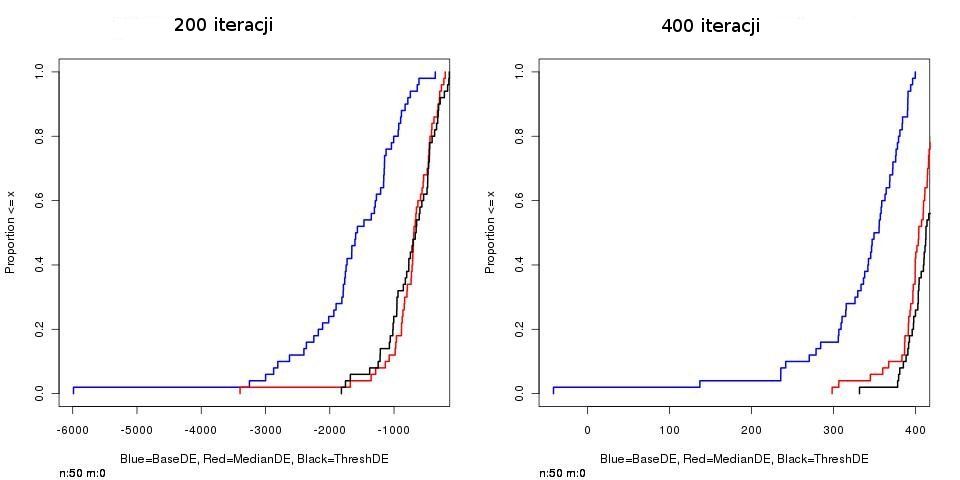
\includegraphics[width=140mm]{cec2005_1.jpg}
\caption{Porównanie modeli selekcji dla funkcji f1}
\label{overflow}
\end{figure}

\subsection{Funkcja f4}
Funkcja f4 jest również funkcją o jednym minimum, ale jej stopień trudności jest większy niż w f1, co wynika to z silnego zaszumienia funkcji celu.
Testy przeprowadzono dla 600 i 900 iteracji.
Wyniki okazały się w obydwu przypadkach podobne do funkcji f1.

\begin{figure}[ht]
\centering
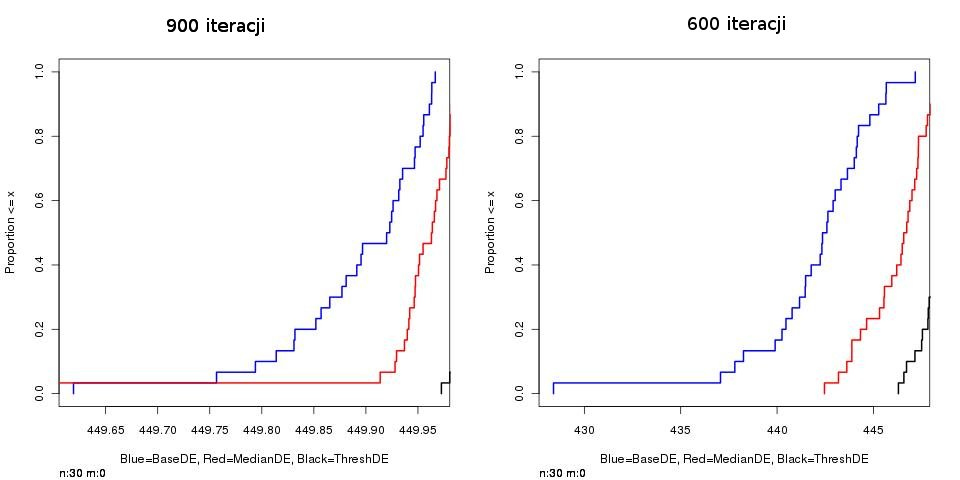
\includegraphics[width=140mm]{cec2005_4.jpg}
\caption{Porównanie modeli selekcji dla funkcji f4}
\label{overflow}
\end{figure}

\subsection{Funkcja f9}
Ponieważ wyniki poprzednich eksperymentów okazały się obiecujące, należało skonfrontować je z trudniejszym problemem.
Przykładem trudnej w optymalizacji funkcji jest niewątpliwie f9, która posiada bardzo dużą liczbę minimów lokalnych.

Funkcja okazała się niestety bardzo trudna nawet w 10 wymiarach, więc do uzyskania reprezentatywnych wyników konieczne było znaczne ograniczenie zakresu dziedziny.
Wyniki dla 1000 iteracji algorytmu nie wskazują na jakiekolwiek różnice pomiędzy modelami selekcji.
Być może większa liczba iteracji byłaby bardziej reprezentatywna, ale czas trwania testów przedłużyłby się ponad standardy projektu akademickiego.

\begin{figure}[ht]
\centering
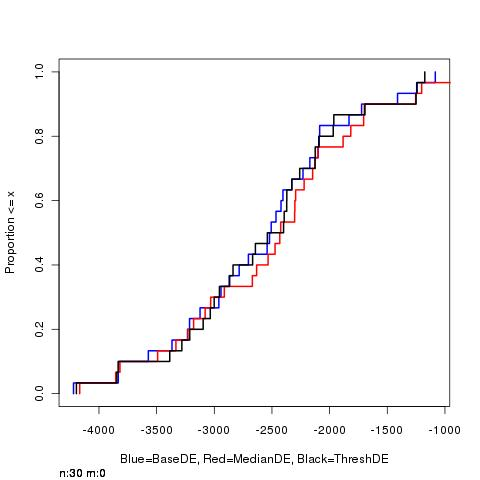
\includegraphics[width=80mm]{cec2005_9.jpg}
\caption{Porównanie modeli selekcji dla funkcji f9}
\label{overflow}
\end{figure}

\section{Wnioski}
Liczba przeprowadzonych testów nie jest wystarczająca do formułowania całościowych wniosków na temat badanych metod selekcji.
Można niemniej zauważyć, że dla funkcji prostych takich jak f1 i f4 zaobserwowano widoczną poprawę szybkości dochodzenia do minimum globalnego.
Z kolei funkcja f9 nie pokazała żadnych różnic pomiędzy metodami selekcji, gdyż posiadała wiele lokalnych minimów.

Wydaje się, że ciekawe mogłoby być przeprowadzenie testów dla znacznie większej populacji np. 100 osobników.
Dałoby to szanse na pełniejsze wykorzystanie selekcji medianowej i w konsekwencji uzyskanie różnic nawet dla trudniejszych funkcji celu.

Dobrym pomysłem do dalszych eksperymentów wydaje się wprowadzenie nieliniowości w obydwu modelach.
Kwadratowa aproksymacja funkcji gęstości prawdopodobieństwa, zwiększyłaby presję na wybór lepszych punktów w końcowej fazie algorytmu.

\end{document}
